\def\year{2015}
%File: formatting-instruction.tex
\documentclass[letterpaper]{article}
\usepackage{graphicx}
\usepackage{aaai}
\usepackage{times}
\usepackage{helvet}
\usepackage{courier}
\frenchspacing
\setlength{\pdfpagewidth}{8.5in}
\setlength{\pdfpageheight}{11in}
\pdfinfo{
/Title (Group Anomaly Detection using Hierarchal Model)
/Author (Put All Your Authors Here, Separated by Commas)}
\setcounter{secnumdepth}{0}  
 \begin{document}
% The file aaai.sty is the style file for AAAI Press 
% proceedings, working notes, and technical reports.
%
\title{Formatting Instructions \\for Authors Using \LaTeX{}}
\author{AAAI Press\\
Association for the Advancement of Artificial Intelligence\\
2275 East Bayshore Road, Suite 160\\
Palo Alto, California 94303\\
}
\maketitle
\begin{abstract}
\begin{quote}
AAAI creates proceedings, working notes, and technical reports directly from electronic source furnished by the authors. To ensure that all papers in the publication have a uniform appearance, authors must adhere to the following instructions.AAAI creates proceedings, working notes, and technical reports directly from electronic source furnished by the authors. To ensure that all papers in the publication have a uniform appearance, authors must adhere to the following instructions.AAAI creates proceedings, working notes, and technical reports directly from electronic source furnished by the authors. To ensure that all papers in the publication have a uniform appearance, authors must adhere to the following instructions.AAAI creates proceedings, working notes, and technical reports directly from electronic source furnished by the authors. To ensure that all papers in the publication have a uniform appearance, authors must adhere to the following instructions.AAAI creates proceedings, working notes, and technical reports directly from electronic source furnished by the authors. To ensure that all papers in the publication have a uniform appearance, authors must adhere to the following instructions. 
\end{quote}
\end{abstract}

\section{Introduction}
Anomalies are data point that don't confirm to the pattern in the data. In most Anomaly detection problem, the idea to identify these point anomalies from the normal data points individually. \\
However, in some applications finding unusual distinction of group of points are crucial. Group anomalies appear when a set of points collectively becomes anomalies. This could happen in three cases, one is when all of the points in the group are anomalies. Another could happen when the group is a mix of normal and anomalies points which lead to unusual distribution of the group. A more interesting case and harder part could be when the group of points are normal individual, but their distribution as a group is unusual. \\

Our motivational domain is finding a threat in an organization based on the users behavior from a fictitious corporate organization, Vegas. The dataset consists of the whole month activities of individual user in the organization. The problem is to find a threat user based on his/her whole month activities. An interesting problem appear when a user activity is normal per day to day bases but could happen unsual compared to other users when his whole month activity are treated collectively. Similar problem could exist in the case of weather data, when a partially broken temperature sensor (e.g. broken sun shield) could apparent to give correct readings . But, when the readings of the station is grouped with its nearby stations on a specific time frame readings bases, the faulty group of reading could be identified.\\

To solve this group anomaly detection, we employ a hierarichal model proposed on [1]. The idea is to exploit a generative model based on LDA extension for the data generation. Where individual data points come from one of the several topics. A group consists of a mix of topics (points). We expect the model to find anomalies group where the topic distribution is abnormal, but the members in the group could be normal.  \\

The paper structured as follows. In section 2 we explain related work. We formally define the proposed hierarchal model in section 3. Then in section 4 we explain the inference for the model. Experimental results starting from synthetic data, ADAMS dataset and Weather data are shown in section 5. Finally, conclusion is given at section 6. \\
\section{Related Work}
Most existing work on group anomaly detection focuses on point-based anomalies detection [1]. A common way is first to find the point anomalies then aggregate the anomalies score of groups. This doesn't work well when the individual points are normal but their group distribution is unsuall, our first experiment on synthetic dataset show the result using this method for Gaussian Mixture Model (GMM). 

For, the group anomaly based detection, the most recent related work is done by[xiliong] based on.The Flexible Genre Model (FGM) [xilong 2011] employs the same idea of the Mixture of Guassian Mixture Model (MGMM). In the model they use a flexible two levels of laten variable to describe a group. At the group level, flexible 'genre' is used to characterize the topic distribution. point level, each point has  
\section{Proposed Model}
\section{Inference}
\section{Experiments}
\subsection{Synthetic dataset}
Gaussian Mixture Model (GMM) using synthetic dataset. We generated synthetic dataset using the generative described in [section 1]. For our experiments we used dataset with 2, 5 and 10 dimension of 50 groups and 5000 points. Then we inject two types of anomalies points. The first types are point wise anomalies with distribution of $ \mathcal{N} (0,1) $ and the second types are group type anomalies with different mean and covariance matrix from the normal group points. Then we assign group different group membership to identify their groups.
To compare the accuracy of the point wise anomaly detector GMM with the MGMM, fist we compute individual likelihood using the GAMM, then we aggregated the score of individual points in the same groups. We took log sum of the score of each points to get the group wise likelihood for the GMM.  Then, we compare the result with the score of group likelihood generated from the MGMM of the 50 groups. The overall performance comparison is shown below.
\begin{figure}
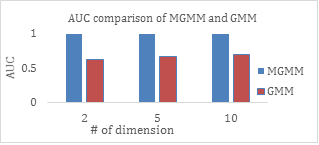
\includegraphics{synthetic.png}
\caption{AUC of group anomaly detector( MGMM) with point anomaly detector (GMM)}
\end{figure}
The result shows, the group anomaly detection achieved better result in all of the dimension dataset compared to the point wise Gaussian mixture Model. 
\begin{figure*}[t]
\begin{center}
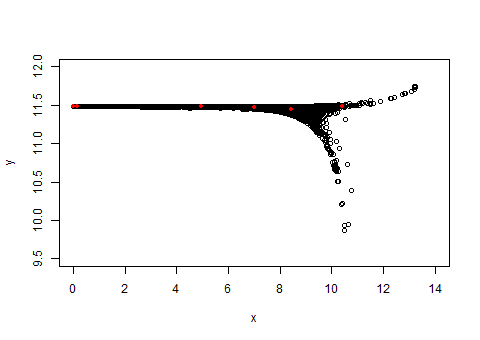
\includegraphics[bb = 0 15 460 290,clip=true,scale=0.9]{Topics.png}
\end{center}
\caption{Scatter plot of all the points along with the 6 topic centers learned (Red points)}\label{learnedTopics}
\end{figure*}

\begin{figure*}[t]
\begin{center}
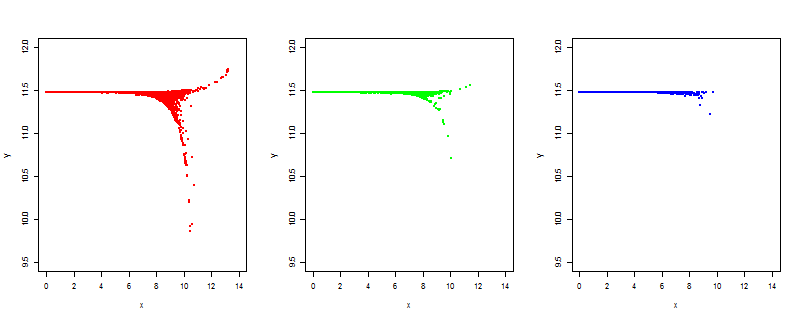
\includegraphics[bb = 0 5 785 285,clip=true,scale=0.65]{Groups.png}
\end{center}
\caption{Scatter plot of the points assigned to group type 1 (left), group type 2 (center) and group type 3 (right)}\label{learnedGroups}
\end{figure*}

\subsection{ADAMS Intrusion Detection Dataset}
This dataset contains information of 5691 users of a corporate network. All activities of these users are monitored and en-coded into 69 features. The activities were recorded by date i.e. for each day we have one feature vector corresponding to one user, which we can call a user day. We run the group anomaly detection on a collection of such user days for the month of April 2013. The complete dataset contains around 170K user day instances. Our goal is to identify the anomalous users i.e. the users those are actually threat. The ground truth anomalies were inserted by the Red Team Inserts, a team whose job is to insert anomalies in a realistic way to make them appear as they occurred naturally. To run the group anomaly detector we treated each user is a group where each group i.e. user contains 30 user days. Our goal is to detect users whose user day distribution appears anomalous i.e. to detect the groups those distributions are different than normal groups distributions. The point here is that the individual user days might not be anomalous but when considered as a group they might appear normal.

We assume that each user group is coming from T normal group types where under each group the user days belongs to one of the K global topic those are shared among the entire dataset.

\subsubsection{Data Preprocessing:}
It is common to apply some dimensionality reduction techniques to the data before applying the anomaly detection, since the dataset might contain some low variance and redundant dimensions. We used PCA to reduce our data. First, we applied PCA and retained only the principle components those represent 95\% of the variance and it reduced the dataset from 69 dimension to just 2 dimensions. We also tried retaining 99\% variance, which reduced the data dimension to 4. And also before applying PCA we scaled the data to have unit variance and then applied the PCA, which reduced the dimension 69 to 38. We run the group anomaly detection on these three reduced datasets and observed that they produce almost similar performance in terms of AUC. Hence, we only report and discus the results found from the reduced 2D data, since it will allow us to get more insight into the datasets.


\subsubsection{Topics and Groups learned:} We choose different values of T and K and computed the corresponding AUC. We got the best AUC of 0.78 when used T = 3 and K = 6, i.e. 3 normal group types and 6 topics. First we show the scattered plot of the reduced 2D dataset in Figure \ref{learnedTopics} along with the 6 topic centers (red dots) found after learning the parameters. It is worth to mention that we translated the points to make all the coordinates positive and then applied log on both x and y axis, hence the x and y axis in Figure \ref{learnedTopics} are in logarithmic scale.

We inferred the group types for each of the users from the learned parameters. We show the data points assigned in three normal group types in figure \ref{learnedGroups}. We observe that most of the groups are assigned to group type 1 and less number of groups are assigned to group type 3.

In figure \ref{distTopic} above we show the distribution of topics under each group types. We see that most of the points are generated from topic 1 and topic 6 and only a few points are generated from topic 2. Group type 3 is sparse i.e. contains most of the points from topic 1 and 6 and almost none from other four topics.

\begin{figure*}[t]
\begin{center}
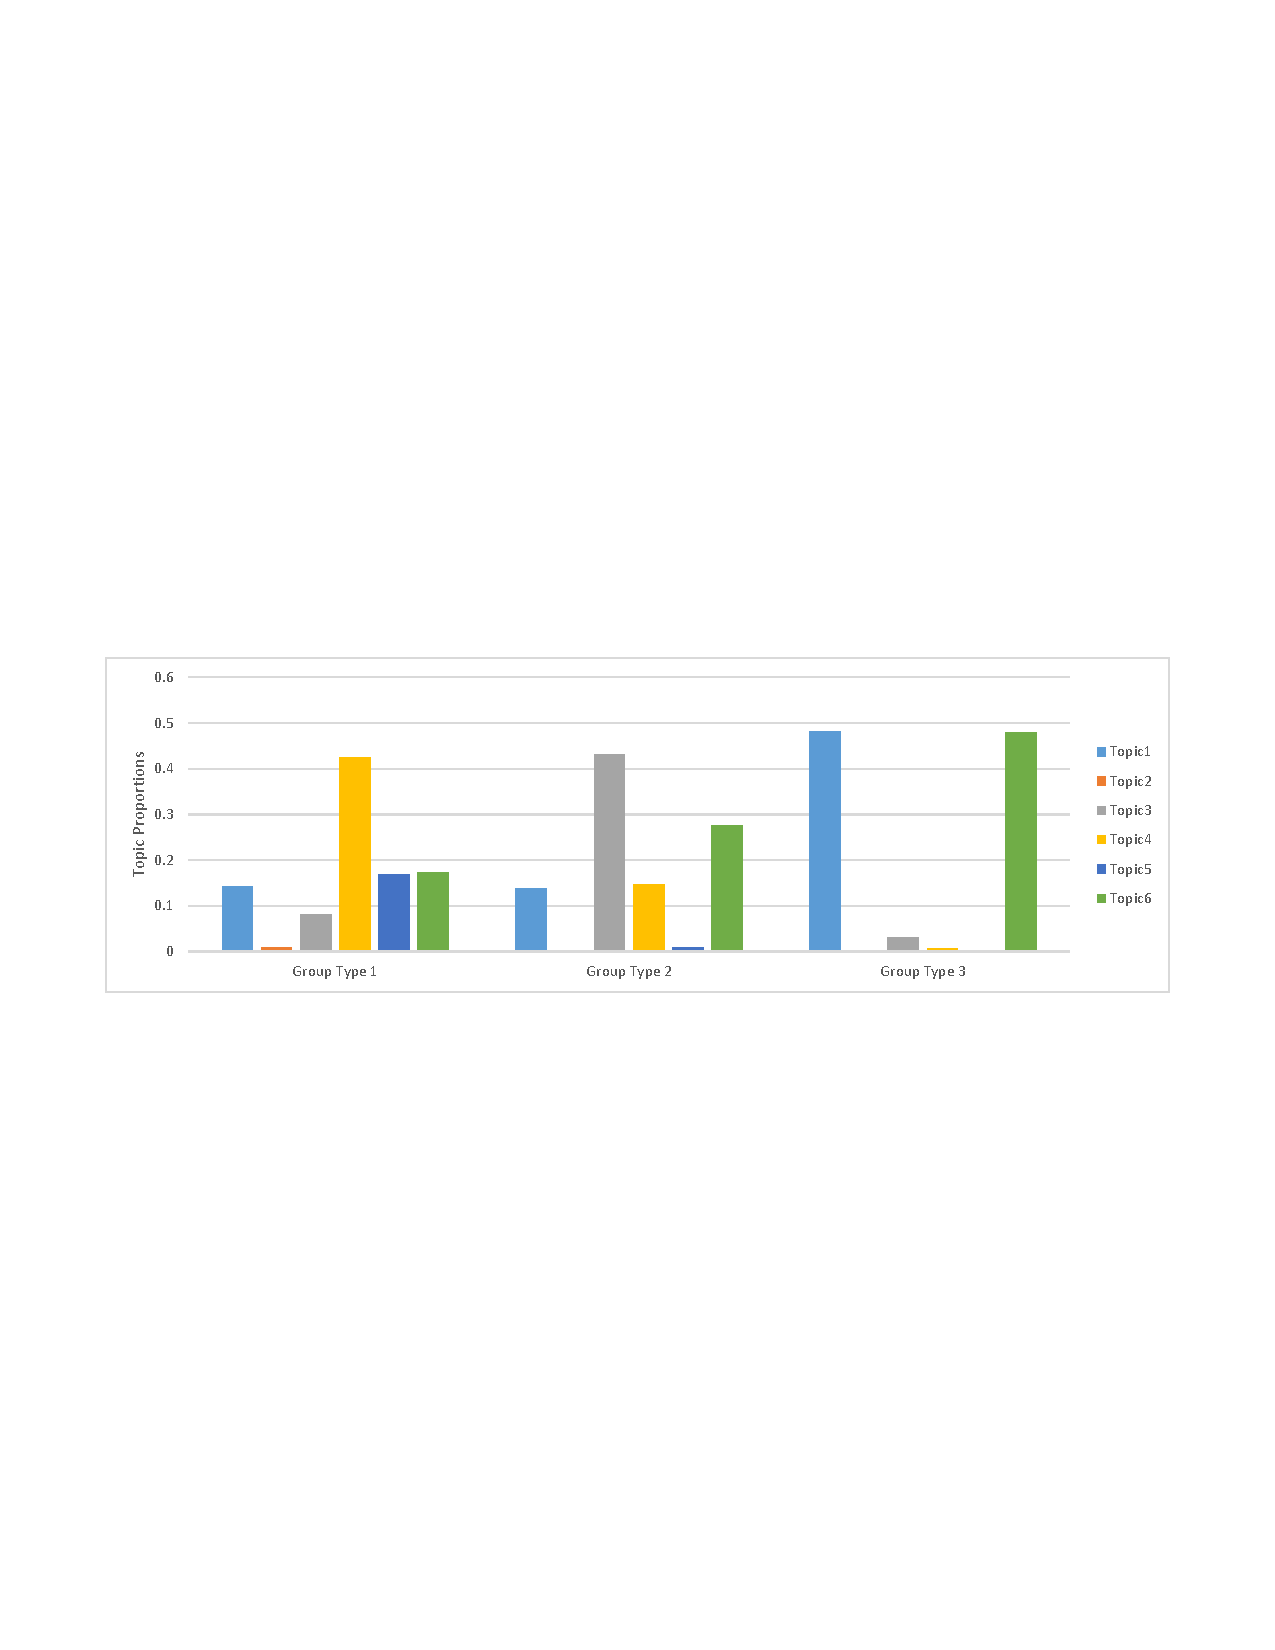
\includegraphics[bb = 55 320 560 470,clip=true,width=1\textwidth]{T3_K6_Chi.pdf}
\end{center}
\caption{Distribution of topics under each groups}\label{distTopic}
\end{figure*}


\subsubsection{Effect of number of normal groups:} We want to see how the performance of the anomaly detector varies when we choose different number of normal group types. In figure \ref{effectGroups} we plot the number of normal groups in x axis and in y axis we put average AUC of different topics.

We observe that in figure \ref{effectGroups}, when we increase number of groups there is a decrease in performance, i.e. AUC decreases and best performance is achieved when using number of normal group types equals 2. The performance degrades when we increase number of normal group types is because anomalous groups will tend to fall under one of these groups which will give more false negatives.

\begin{figure}[t]
\begin{center}
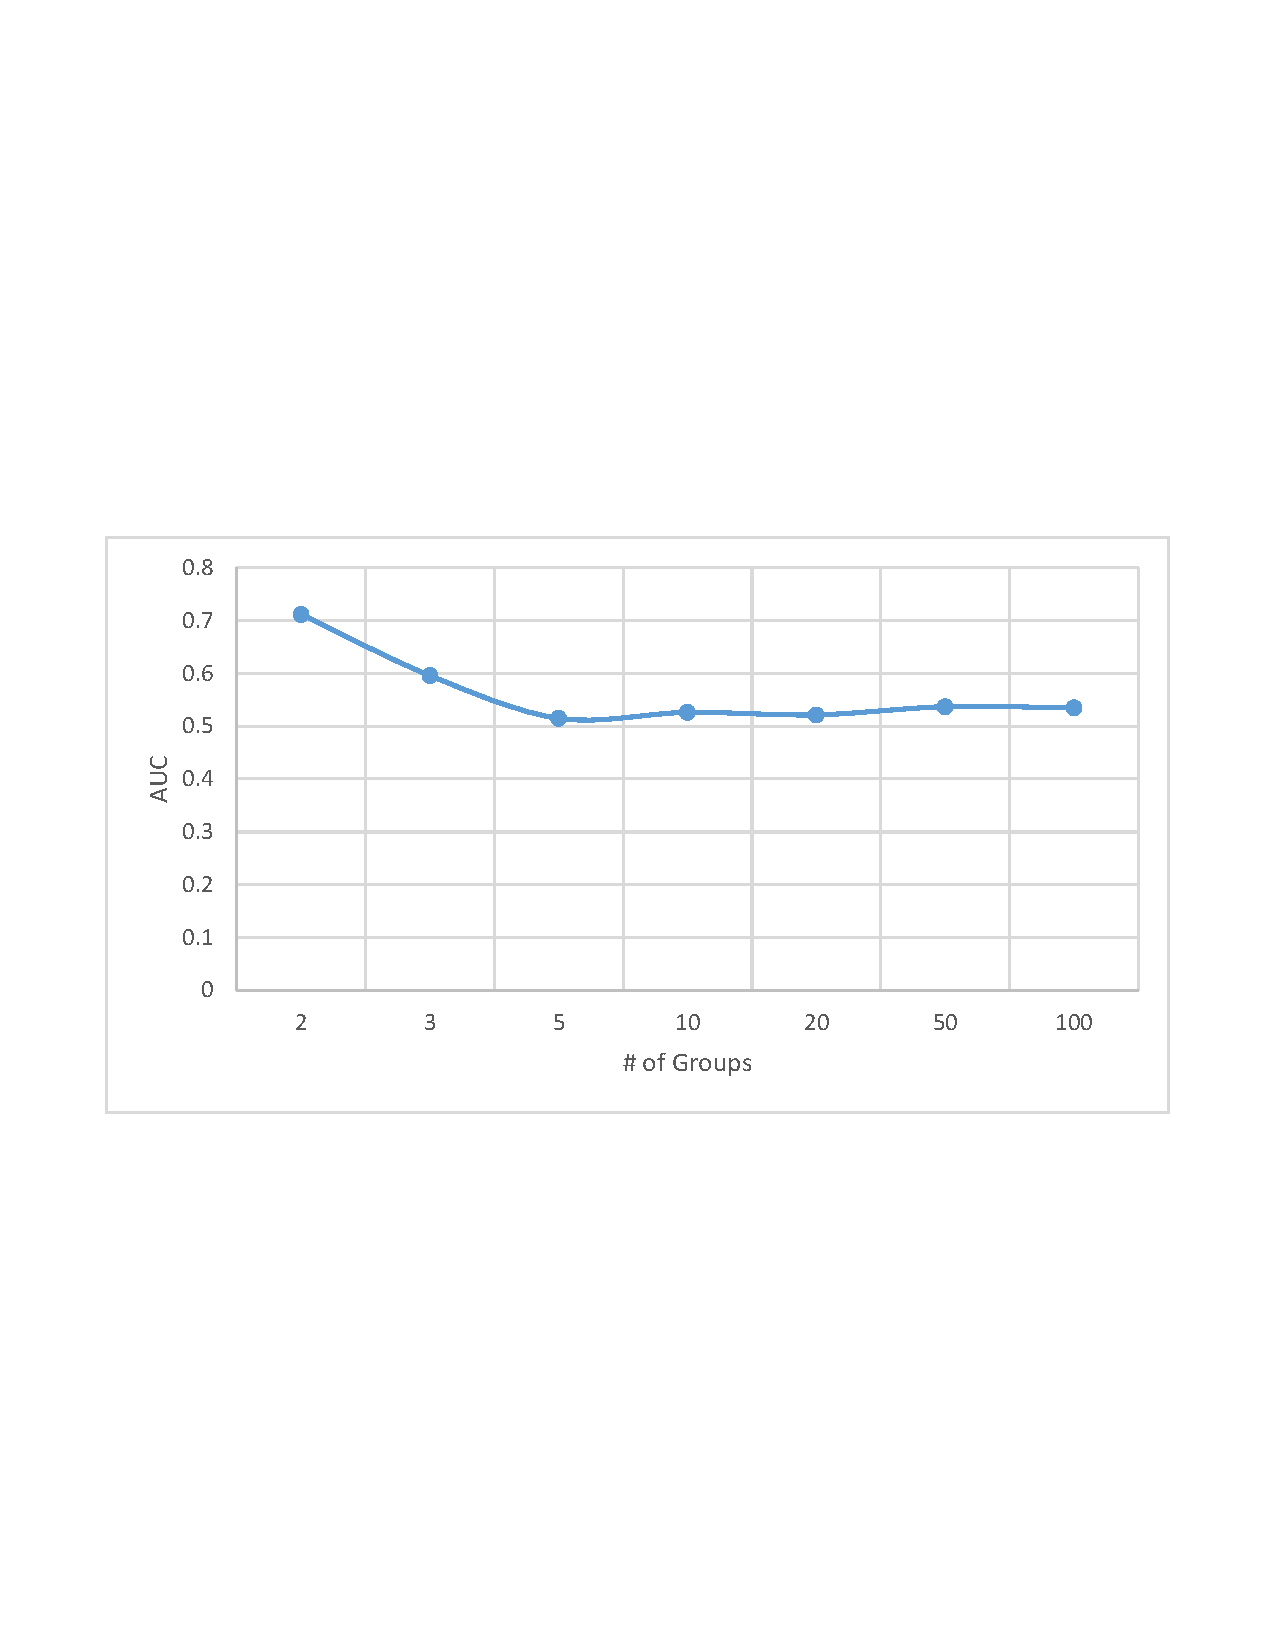
\includegraphics[bb = 70 270 550 530,clip=true,width=0.45\textwidth]{ResultGroupVsAUC.pdf}
\end{center}
\caption{Effect of number of groups in performance of anomaly detector}\label{effectGroups}
\end{figure}

\begin{figure}[t]
\begin{center}
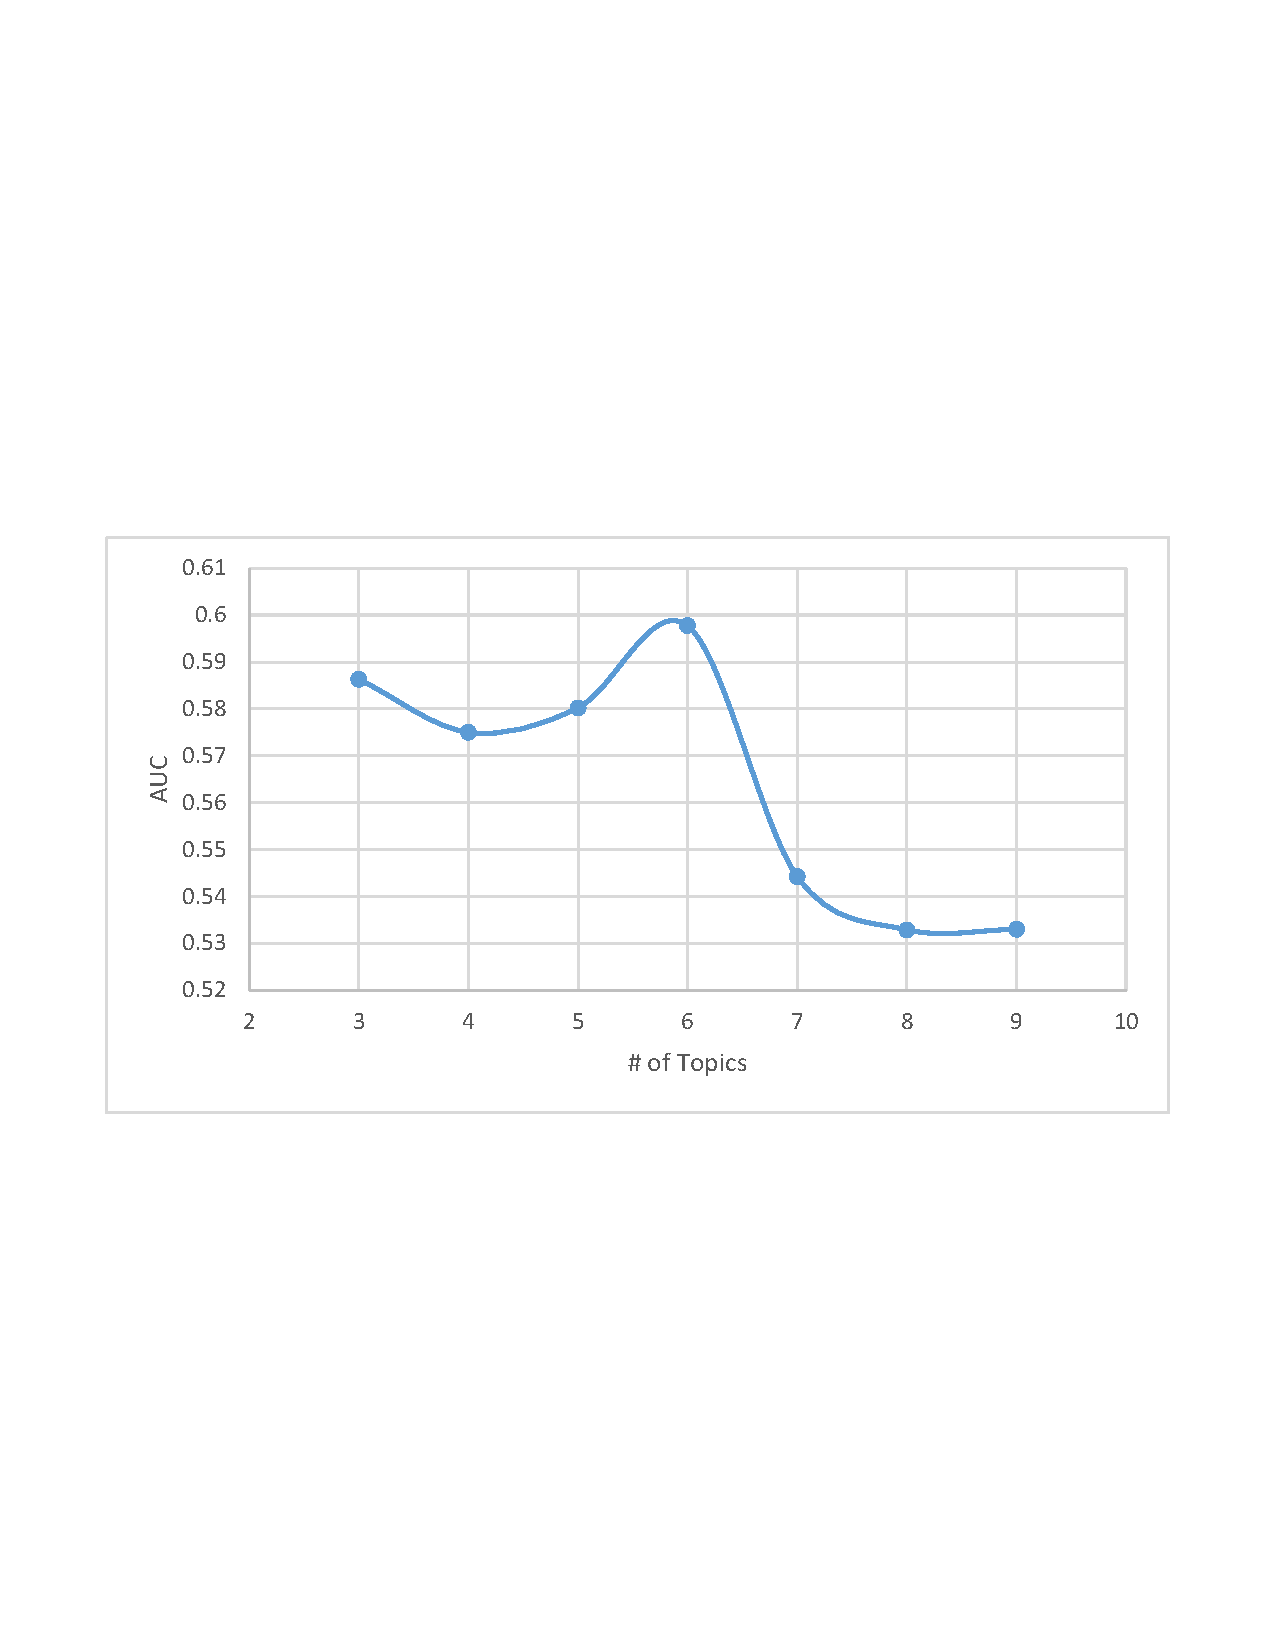
\includegraphics[bb = 70 270 550 530,clip=true,width=0.45\textwidth]{ResultTopicVsAuc.pdf}
\end{center}
\caption{Effect of number of topics in performance of anomaly detector}\label{effectTopics}
\end{figure}


\subsubsection{Effect of number of topics:} In figure \ref{effectTopics} below we plot number of topics vs. average AUC in different group numbers. Choosing small number of topics does not help identifying anomalous groups. Also large number of topics does not. We observed that the best performance is achieved when number of topics is 6. The reason is that when we have very small number of topics the group types will tend to produce similar topic distributions hence will get lots of false negatives, on the other hand if we have large number of topics the distributions will be mostly anomalous and will produce large number of false positives. In both of the cases the anomaly detector will perform badly.
\subsection{Weather temperature dataset}
In this experiment, we tested the performance of the group anomaly detection in air temperature weather data from Oklahoma state weather stations. The weather station have every 5 minutes readings which constitute 288 readings in each day. In our case we are interested in whole day readings of 288 dimensions.\\
 In order to prepare dataset for group anomaly detection problem, first we selected 12 weather stations which are not far apart. We chose a sample weather station i.e. 'SPEN', then we collect data from all weather station which are under 40 miles radius from it. Our assumption is, stations which are close to each other will have highly correlated readings in specific time instance. For example, in a particular day and time, each station will have similar readings. Using this assumption, we proposed a grouping method based on days, where each group contains readings from all station in the particular day. So, we formulate total 365 groups for the 12 weather stations proposed.\\
 Then anomalies points happen when there is failure in a particular weather station. So, a group can be anomaly if it has one or more faulty readings from its station in that day. Here our objective is to detect these anomalies group (days) by exploiting the grouping structure of the readings. To perform that first we reduced the dimension of the data using PCA from 288 to 4 dimension by retaining 95\% variance of the features . The problem with the original dimension it was intractable for our model to learn it and we assume also there is low variance in the features.  \\
We tested our proposed hierarchal model on this domain to find the likelihood score of each groups using different topic and group type proportion.  Our assumption is if there is a faulty readings from one station in particular day, this will make the group likelihood low. For the experiments we used different parameter set of Topic and group type, T=2, 3, 5, 10, 20 and 100 and K= 3 to 7.  The performance is measured using area under the ROC curve (AUC) of finding the anomalies from the test set.  For the ground truth of the dataset we used the label for each day readings of a particular station.  To generate ground truth for the groups, we assumed if there is one or more faulty stations in that day the group is flagged as faulty.\\  
The overall result shows, detection performance of the models is not really good. There reason could be because in the dataset the number of group members are small. For example, in this dataset in each group we have 12 points from the 12 weather station. The performance might be increased if we increase number of stations. But, increasing number of station with further distance might decrease the correlation as well, which leads to an informative grouping. But, in comparison the algorithm achieves better for Topic proportion of T=5 and group type K=4. In other hand, the result in the weather data shows, after certain topic configuration, the accuracy tends to decrease as we increase number of topics or group type. \\
\begin{figure}
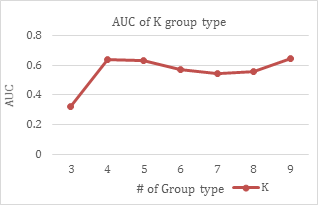
\includegraphics{grouptype.png}
\caption{AUC comparison of different group type}
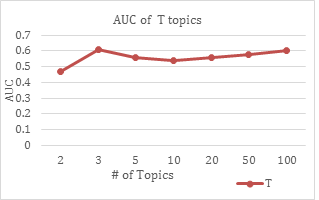
\includegraphics{topic.png}
\caption{AUC comparison of different topic type}
\end{figure}

Then from the AUC result we took the better result for group type K=4 and topics T=5 which is around 0.71. Us-ing this configuration we compute the topic proportion of each group type, which is shown in the figure below.
\begin{figure}
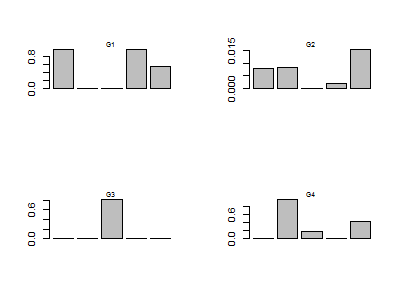
\includegraphics[scale=0.6]{topicprop.png}
\caption{AUC comparison of different group type}
\end{figure}
The result figure shows, how each group type are different in their topic composition. For example, Group type 1 are mostly from topic 1, 4 and 5, and Group type 3 are mostly composed of topic 3. 
\section{conclusion}
\section{Reference}
\end{document}
